\hypertarget{(chap:capitolo6)}{}
\chapter{Risultati sperimentali}
In questo capitolo andremo a vedere i risultati sperimentali per ogni metodo.
\section{Risultati preprocessing matrici grezze}
Nelle sezione successive andremo a vedere i risultati delle valutazioni di ciascun modello rispetto la metrica $AUC$ e la $NDCG$ con $k\in \{5, 10, 25, 100\}$, in particolare la metrica che riteniamo sia più significativa è la seconda in quanto si basa sul ranking degli item nella lista $TopN$. \\
Per i confronti abbiamo scelto di usare $NDCG$ con $k=25$. Nei seguenti grafici

\subsection{Risultati base}
In questa sezione andremo a vedere i risultati del modello MostPop e del VAECF, che verranno utilizzati come bound per valutare quelli succcessivi. 

\subsubsection{MostPop}
Come detto il modello MostPop restituisce per ogni user la stessa lista di item più popolari.
Andiamo a vedere i risultati per dataset sul validation set:\\

\begin{tabular}{|l|c|cccc|}
    \toprule
    $dataset$ &    $AUC$ &  $NDCG@10$ & $NDCG@100$  & $NDCG@25$ & $NDCG@5$  \\
    \midrule
    macchine & 0.7644 & 0.1263 &   0.2414 &  0.1647 & 0.0920 \\
    ricambi  & 0.3427 &  0.0299 &   0.0732 &  0.0358 & 0.0000 \\
    totale  & 0.2810 &  0.0733 &   0.0811 &  0.0627 & 0.0360 \\

\bottomrule
\end{tabular}\\

Useremo questi risultati come bound per quelli degli altri modelli (MF, UserKnn), nel caso in cui questi siano migliori si procederà al tuning dei parametri e al calcolo finale dei risultati sul test set.\\
Quelli riportati qui di seguito sono i risultati del MostPop sul test set.\\

\begin{tabular}{|l|c|cccc|}
    \toprule
    $dataset$ &    $AUC$ &  $NDCG@10$ & $NDCG@100$  & $NDCG@25$ & $NDCG@5$  \\
    \midrule
    macchine & 0.7897 &  0.1364 &   0.2610 &  0.1875 & 0.1001 \\
    ricambi  & 0.3924 &  0.0753 &   0.1365 &  0.0793 & 0.0619 \\
    totale  & 0.3101 &  0.0807 &   0.1281 &  0.0866 & 0.0944 \\

\bottomrule
\end{tabular}

\subsubsection{VAECF}
Il modello VAECF è un modello che funziona su rating impliciti, la fase preliminare ha richiesto il tuning dei parametri riportati di seguito:
\begin{itemize}
    \item $n_{int}$ è la dimensione della rappresentazione latente interna, i possibili valori sono $\{5,10,15,20,50\}$;
    \item $n_{hid}$ è il numero di neuroni del layer dell'encoder e del decoder, i valori possibili sono $\{10,20,30,50,100,200\}$;
    \item $f_{act}$ è la funzione di attivazione applicata nei layer nascosti, che può essere una delle seguenti $\{sigmoid, tanh, elu, relu, relu6\}$.
\end{itemize}
\begin{minipage}[H]{0.45\textwidth}
    \begin{tabular}{|l|ccc|}
        \toprule
        $dataset$ &    $n_{int}$ &  $n_{hid}$ & $act\_f$ \\
        \midrule
        macchine & 5 & 30 & relu \\
        ricambi  &	5 & 30 & sigmoid\\
        totale  & 5 & 30 & sigmoid\\
    \bottomrule
    \end{tabular}\\
\end{minipage}
\begin{minipage}[H]{0.55\textwidth}
    Il tuning dei parametri ha portato a considerare tutte le possibili combinazioni dei parametri sopra citati, andiamo a vedere per ogni dataset quali parametri hanno restituito sul validation set i risultati migliori.
\end{minipage}\\

Andiamo a vedere i risultati per dataset sul validation set dopo il tuning dei parametri:\\

\begin{tabular}{|l|c|cccc|}
    \toprule
    $dataset$ &    $AUC$ &  $NDCG@10$ & $NDCG@100$  & $NDCG@25$ & $NDCG@5$  \\
    \midrule
    macchine & 0.8201 & 0.1768 & 0.3032 & 0.2282 & 0.1325 \\
    ricambi & 0.4773 & 0.0452 & 0.1052 & 0.0643 & 0.0506 \\
    totale  & 0.4190 & 0.0980 & 0.0941 & 0.0741 & 0.1208 \\
\bottomrule
\end{tabular}\\

Dato che i risultati della tabella precedente sono quelli del validation set su un modello con parametri ottimizzati, non possiamo direttamente usarli per il confronto con 

Vediamo i risultati del modello validato sul test set:\\

\begin{tabular}{|l|c|cccc|}
    \toprule
    $dataset$ &    $AUC$ &  $NDCG@10$ & $NDCG@100$  & $NDCG@25$ & $NDCG@5$  \\
    \midrule
    macchine & 0.8269 &  0.1948 &   0.3301 &  0.2487 & 0.1473 \\
    ricambi  & 0.4930 &  0.0919 &   0.1401 &  0.1075 & 0.0801 \\
    totale  & 0.4343 &  0.0874 &   0.1398 &  0.0964 & 0.0988 \\

\bottomrule
\end{tabular}

\subsection{Fase test preliminare}
In questa sezione andremo a vedere per ogni tecnica di preprocessing adottata sulle matrici grezze i risultati ottenuti.
La valutazione si è divisa in due fasi: 
\begin{enumerate}
    \item preliminare: confrontiamo i risultati dei modelli (MF, UserKnn) con parametri di default sulle matrici dei rating, con il risultato bound dato dal MostPop;
    \item avanzata: dopo aver effettuato il tuning sui parametri dei modelli con le matrici rimanenti, si confrontano con il bound dato dal VAECF. 
\end{enumerate} 
Cominceremo prima con la tecnica basata su min-max, poi con quella ordered-based per concludere infine con quella basata sui prodotti totali. 
Spesso si farà riferimenti ai risultati dei modelli, intendendo il risultato dato dei modelli basato sulle diverse matrici dei rating.

%------------------------------------------------------------------------------------------------------------------------------------------------------

\subsubsection{Normalizzazione min-max}
Come spiegato nel capitolo dedicato alle tecniche ora andremo ad osservare i risultati rispetto diversi gruppi di triplette.\\

\paragraph{Gruppo globale}\mbox{} \\
In questa sezione vedremo la normalizzazione min-max applicata al gruppo globale, ossia quello contenente tutte le triplette.
Nella tabella sottostante possiamo vedere sulle righe i dataset (macchine, ricambi, totale), mentre sulle righe possiamo vedere le \textit{espressioni d'interesse}. Ciascun grafico poi mostra sulle ascisse la $scale$ della matrice dei rating e sulle ordinate il risultato ottenuto da tale matrice rispetto la metrica $NDCG@25$. \\
La linea tratteggiata blu rappresenta il risultato del modello MostPop che viene usato come bound.
In questo grafico composto per ogni valore della scala vengono riportati quattro puntini, per questa tecnica ogni matrice dei rating è stata tenuta sia in versione continua che in versione intera, a queste due matrici vengono applicati i modelli MF e UserKnn, da otteniamo quattro risultati, quelli di colore blu sono i risultati forniti dal modello MF, mentre quelli arancioni quelli del modello UserKnn.

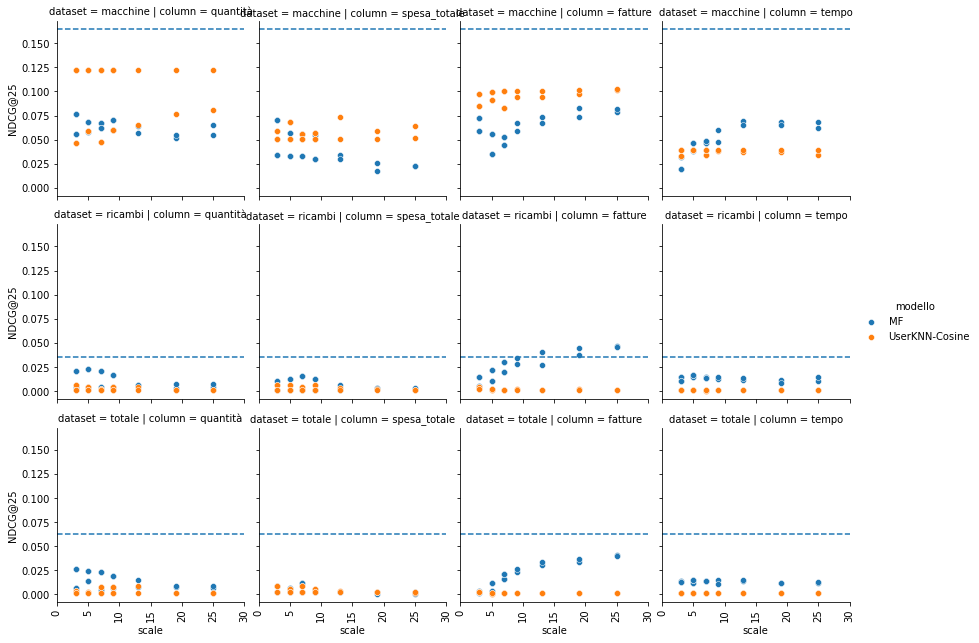
\includegraphics[width=16cm]{figures/risultati_minmax_globale.png}

\paragraph{Gruppi user-based}\mbox{} \\
In questa sezione vedremo la normalizzazione min-max applicata al gruppo user-based, ossia quello dove ciascun gruppo contiene solo le triplette di un singolo user. Il grafico composto di seguito possiede la stessa disposizione di quello del paragrafo precedente.

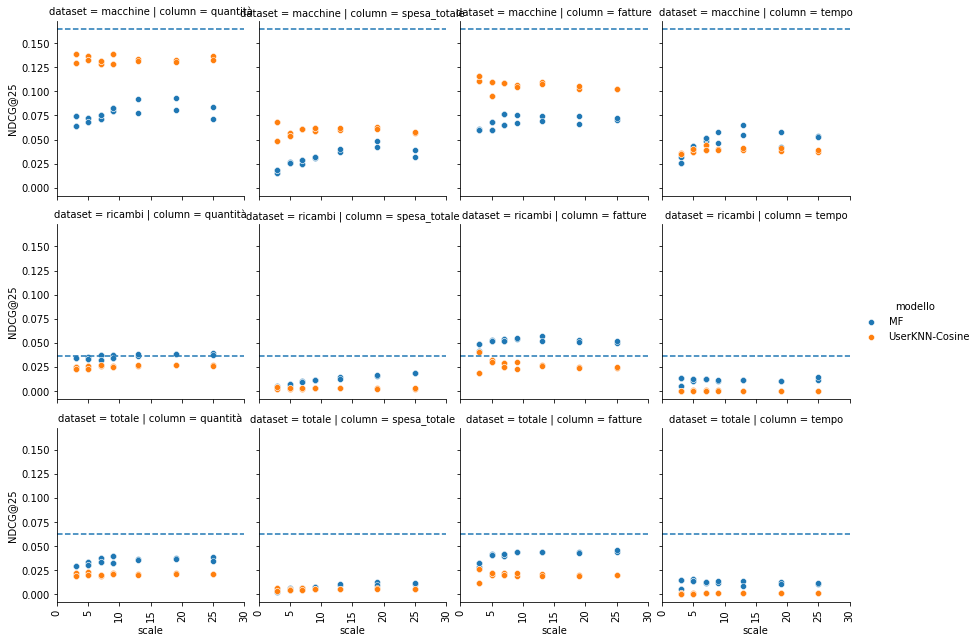
\includegraphics[width=16cm]{figures/risultati_minmax_singolo.png}
\newpage
\paragraph{Gruppo user-category-based}\mbox{} \\
Ora andremo a vedere la normalizzazione min-max applicata però al gruppo user-category-based, dove le triplette vengono divise per user e per categoria.
Le macchine hanno a disposizione solo la divisione in categorie secondo la gerarchia prodotto, mentre i ricambi possono essere divisi secondo le categorie della gerarchia prodotto di 2° e 3° e dal gruppo merceologico. Per il tipo dataset totale si proverà la divisione solo con la gerarchia prodotto, e poi unendo insieme la divisione delle macchine secondo le categorie di ciascun livello e i ricambi divisi secondo il gruppo merceologico.

\subparagraph{Macchine}\mbox{} \\
Come possiamo vedere dal grafico composto, sulle righe abbiamo le categorie una per ciascun livello della gerarchia prodotto (1°, 2°, 3° livello), mentre sulle colonne abbiamo le espressioni d'interesse. Non ci sono risultati sopra la soglia critica. Non sono presenti risultati che superino la soglia critica.\\

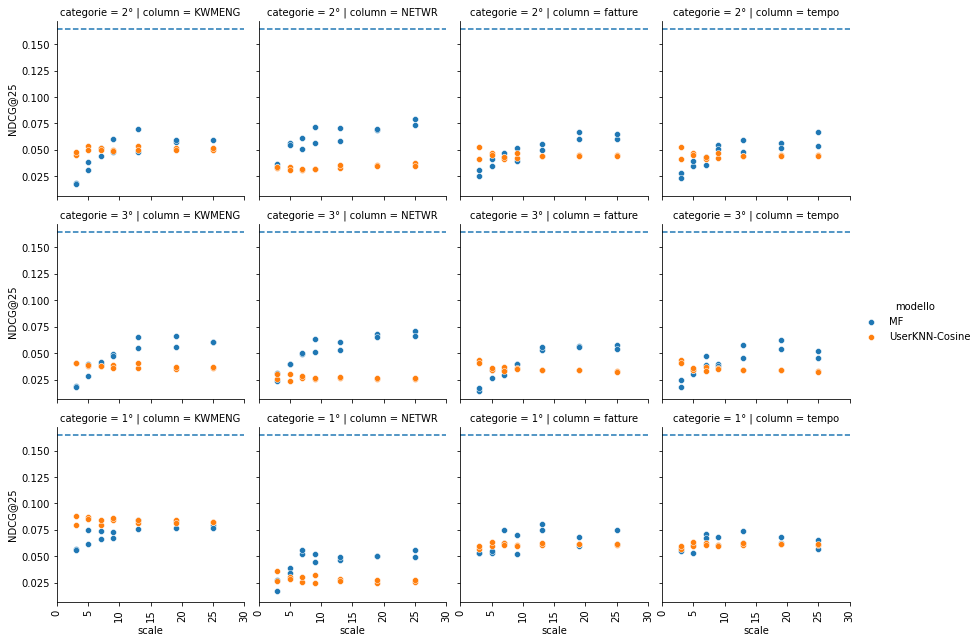
\includegraphics[width=16cm]{figures/risultati_minmax_categoria_macchine.png}
\newpage

\subparagraph{Ricambi}\mbox{} \\
Come possiamo vedere dal grafico composto, sulle righe abbiamo le categorie di 1° e 2° livello della gerarchia prodotto e la divisione del gruppo merceologico matkl, mentre sulle colonne abbiamo le espressioni d'interesse. Abbiamo risultati che superano la soglia critica dividendo le triplette secondo le categorie di 2° livello con le espressioni quantità e recentezza.\\

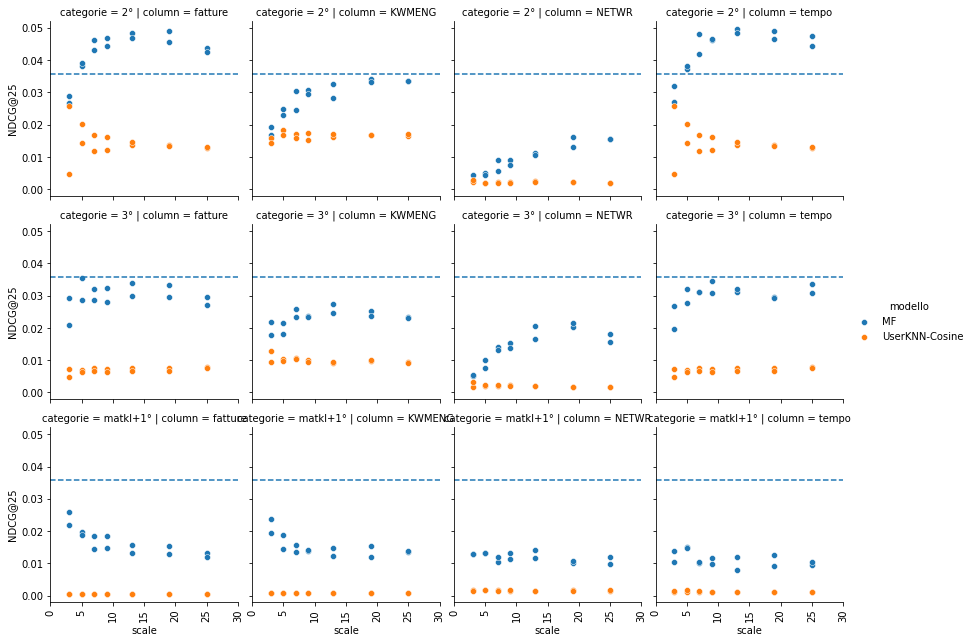
\includegraphics[width=16cm]{figures/risultati_minmax_categoria_ricambi.png}

\subparagraph{Totale}\mbox{} \\
Come possiamo vedere dal grafico composto, sulle righe abbiamo le categoria della gerarchia prodotto 1°, 2° e 3° livello e poi le precedenti categorie applicate solo alle macchine unite al gruppo merceologico per i ricambi. Sulle colonne abbiamo le espressioni d'interesse.\\

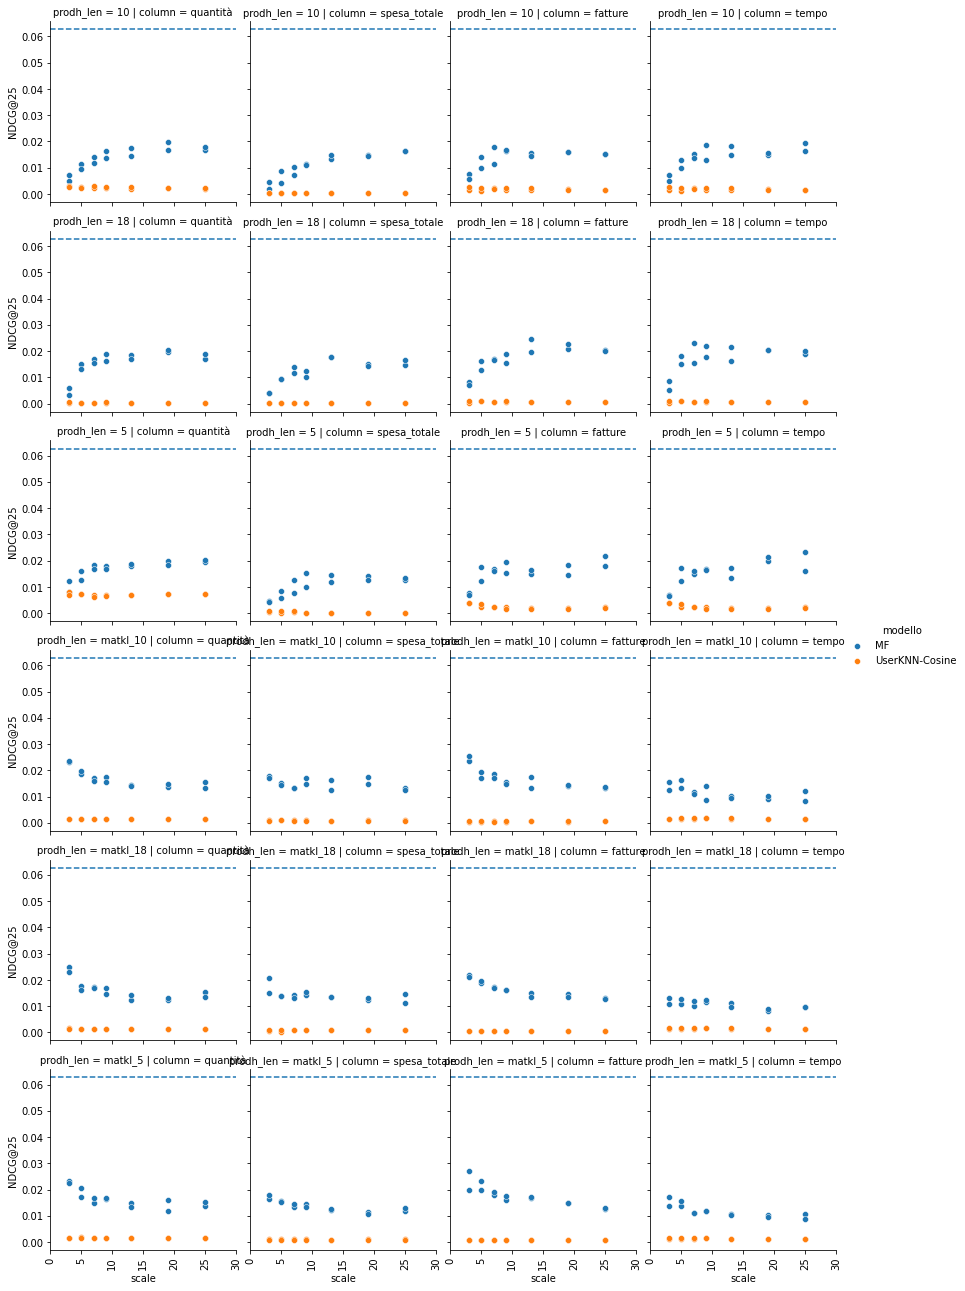
\includegraphics[width=16cm]{figures/risultati_minmax_categoria_totale.png}

%------------------------------------------------------------------------------------------------------------------------------------------------------

\subsubsection{Tecnica ordered-based}

\paragraph{Gruppo globale}\mbox{} \\
In questa sezione vedremo la tecnica di preprocessing ordered-based applicata al gruppo globale, ossia quello contenente tutte le triplette.
Nella tabella sottostante possiamo vedere sulle righe i dataset (macchine, ricambi, totale), mentre sulle colonne possiamo vedere le \textit{espressioni d'interesse}. Ciascun grafico poi mostra sulle ascisse la $scale$ della matrice dei rating e sulle ordinate il risultato ottenuto da tale matrice rispetto la metrica $NDCG@25$. La linea tratteggiata blu rappresenta il risultato del modello MostPop che viene usato come bound.
In questo grafico composto per ogni valore della scala vengono riportati quattro puntini, ogni matrice dei rating durante la fase di creazione può utilizzare una distribuzione uniforme discreta o gaussian-like, a queste due matrici vengono applicati i modelli MF e UserKnn da cui otteniamo quattro risultati, quelli di colore blu sono i risultati forniti dal modello MF, mentre quelli arancioni quelli del modello UserKnn.

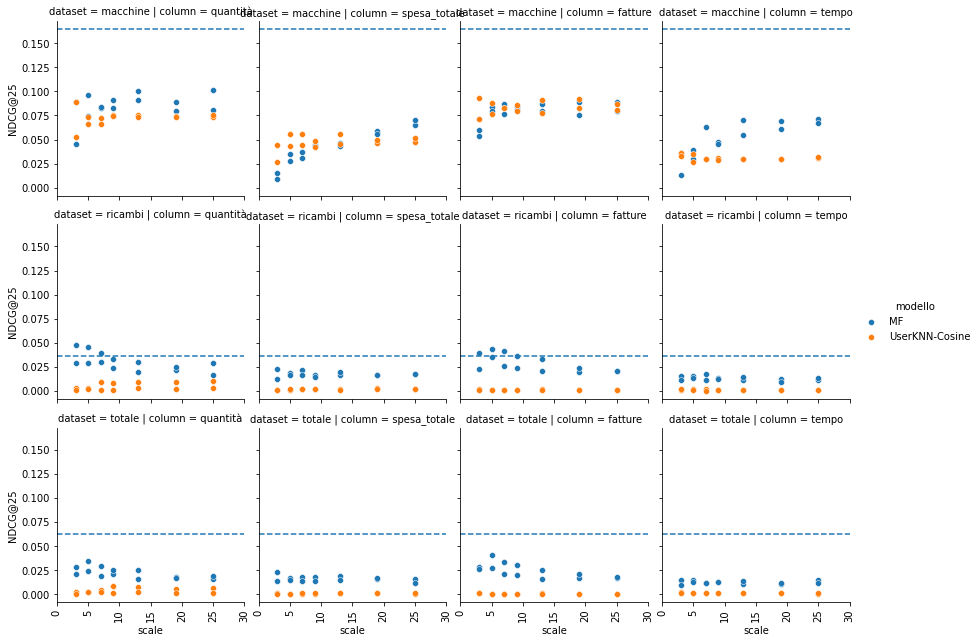
\includegraphics[width=16cm]{figures/risultati_ordered_globale.png}

\paragraph{Gruppi user-based}\mbox{} \\
Di seguito possiamo vedere i risultati relativi la tecnica ordered-based su gruppi di triplette appartenenti allo stesso user.
Il grafico composto di seguito possiede la stessa disposizione di quello del paragrafo precedente.\\

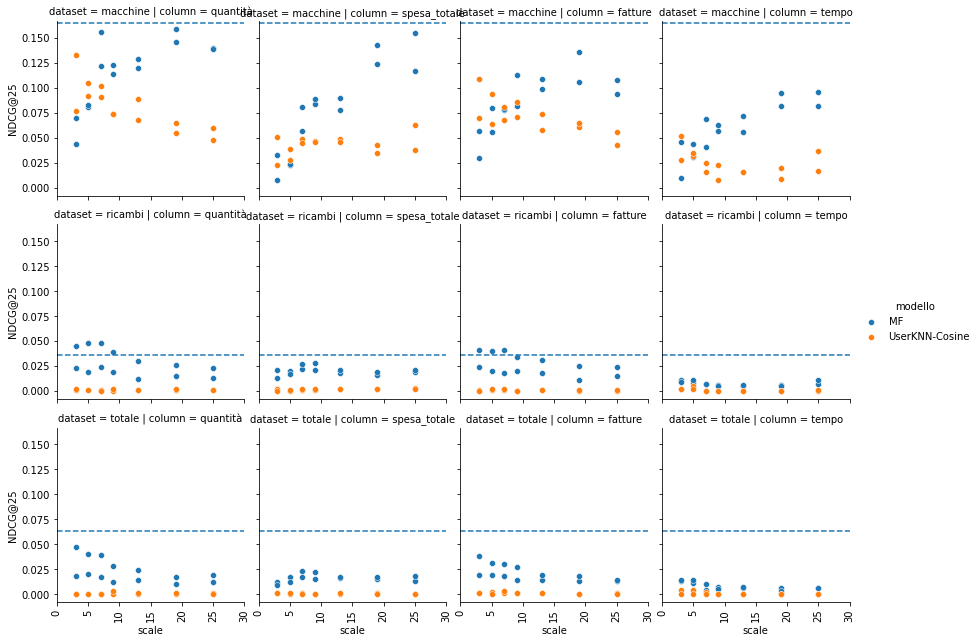
\includegraphics[width=16cm]{figures/risultati_ordered_singolo.png}

\paragraph{Gruppo user-category-based}\mbox{} \\
\subparagraph{Macchine}\mbox{} \\
Come possiamo vedere dal grafico composto, sulle righe abbiamo le categorie una per ciascun livello della gerarchia prodotto (1°, 2°, 3° livello), mentre sulle colonne abbiamo le espressioni d'interesse. Non ci sono risultati sopra la soglia critica. Non sono presenti risultati che superino la soglia critica.\\

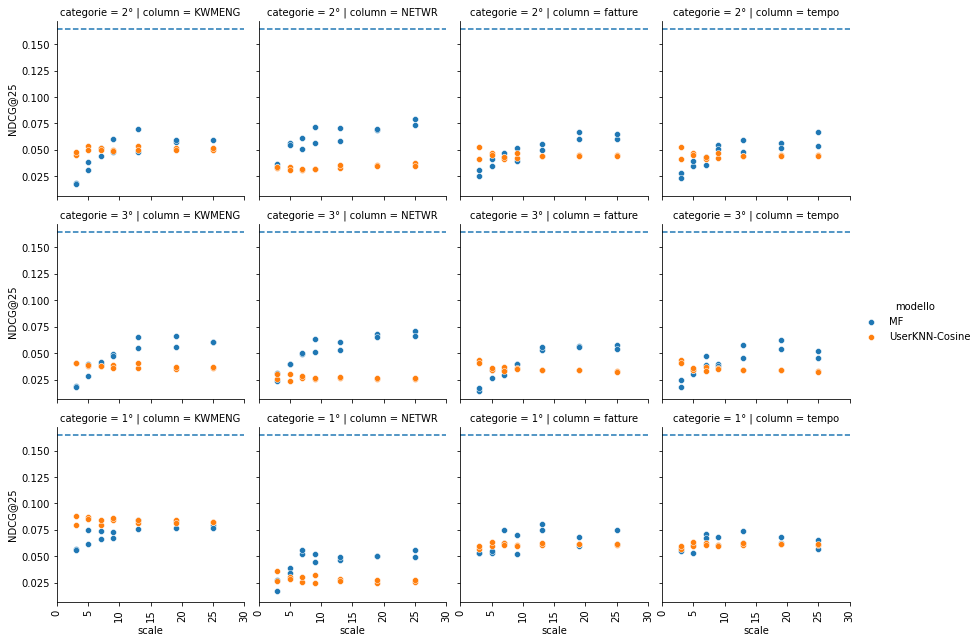
\includegraphics[width=16cm]{figures/risultati_minmax_categoria_macchine.png}
\newpage

\subparagraph{Ricambi}\mbox{} \\
Come possiamo vedere dal grafico composto, sulle righe abbiamo le categorie di 1° e 2° livello della gerarchia prodotto e la divisione del gruppo merceologico matkl, mentre sulle colonne abbiamo le espressioni d'interesse. Abbiamo risultati che superano la soglia critica dividendo le triplette secondo le categorie di 2° livello con le espressioni quantità e recentezza.\\

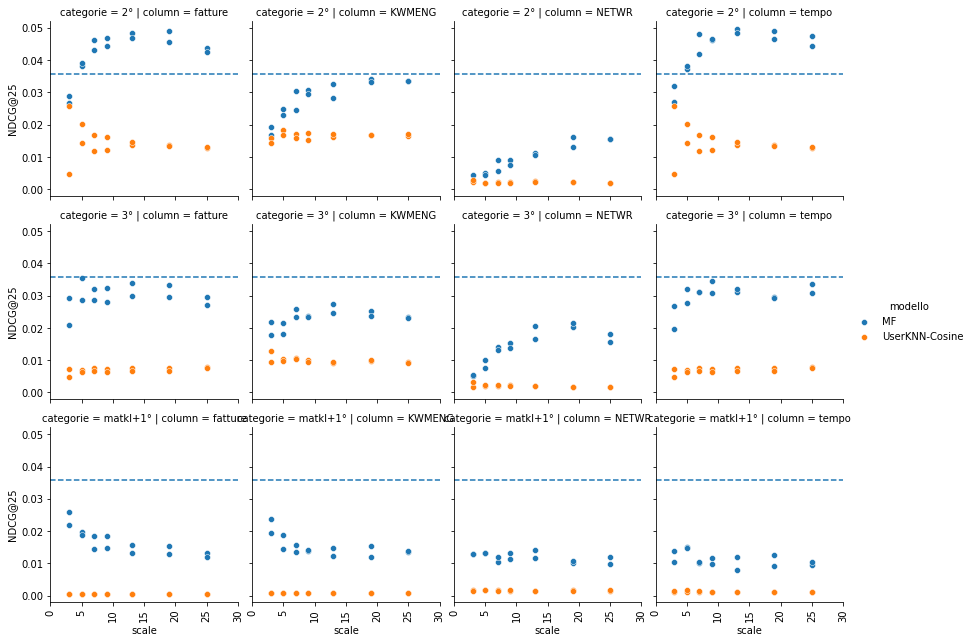
\includegraphics[width=16cm]{figures/risultati_minmax_categoria_ricambi.png}

\subparagraph{Totale}\mbox{} \\
Come possiamo vedere dal grafico composto, sulle righe abbiamo le categoria della gerarchia prodotto 1°, 2° e 3° livello e poi le precedenti categorie applicate solo alle macchine unite al gruppo merceologico per i ricambi. Sulle colonne abbiamo le espressioni d'interesse.\\

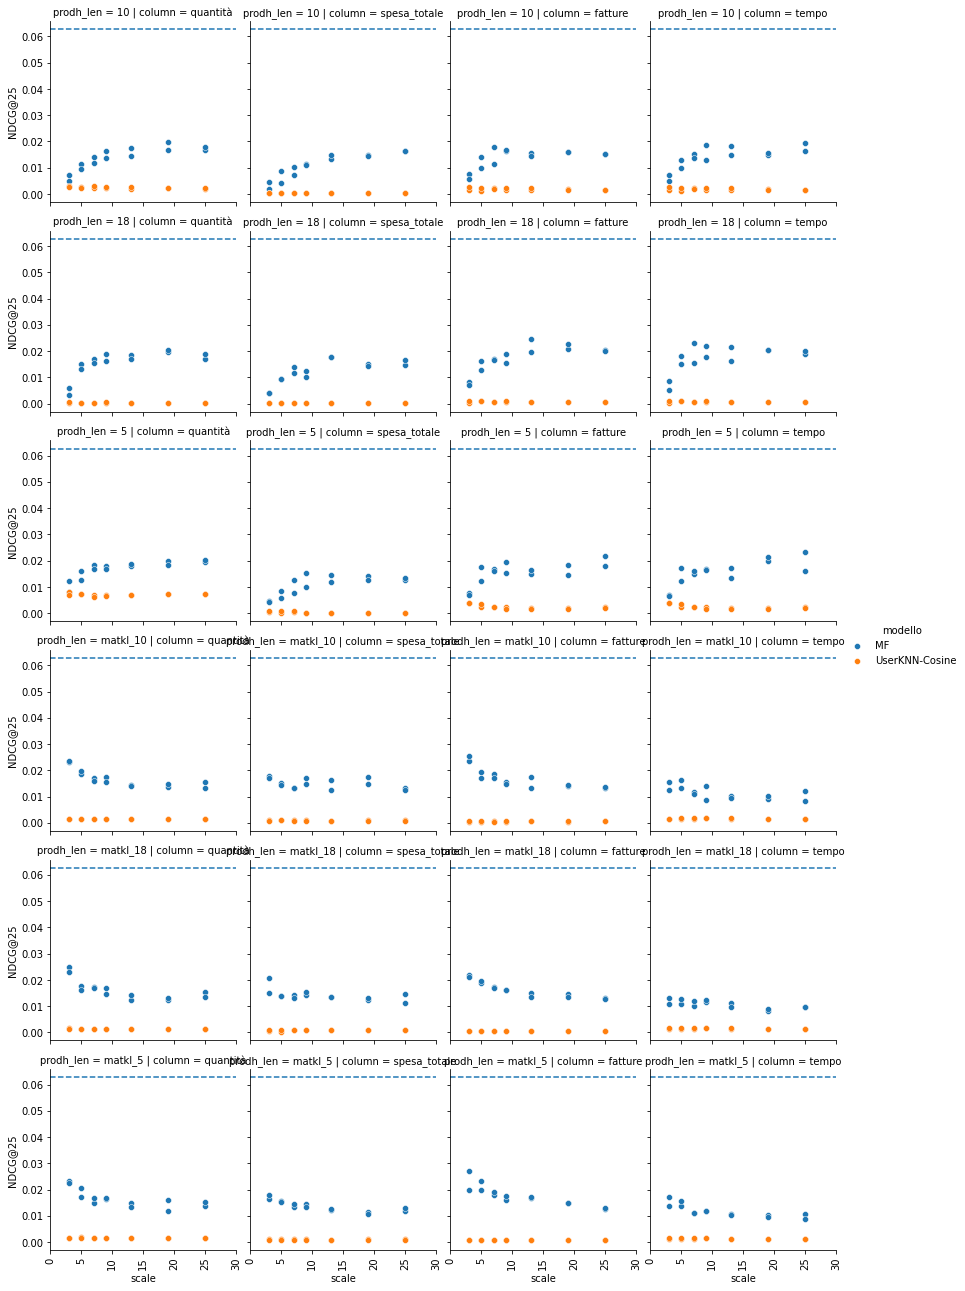
\includegraphics[width=16cm]{figures/risultati_minmax_categoria_totale.png}

%-------------------------------------------------------------------------------------------------------------------------------------------------------

\subsubsection{Tecnica product-based}
In questa sezione vedremo la tecnica di preprocessing product-based, dove si assegna ad ogni item lo stesso rating.
Nella tabella sottostante possiamo vedere sulle righe i dataset (macchine, ricambi, totale), mentre sulle colonne possiamo vedere le \textit{espressioni d'interesse}. Ciascun grafico poi mostra sulle ascisse la $scale$ della matrice dei rating e sulle ordinate il risultato ottenuto da tale matrice rispetto la metrica $NDCG@25$. La linea tratteggiata blu rappresenta il risultato del modello MostPop che viene usato come bound.
In questo grafico composto per ogni valore della scala vengono riportati quattro puntini, ogni matrice dei rating durante la fase di creazione può utilizzare una distribuzione uniforme discreta o gaussian-like, a queste due matrici vengono applicati i modelli MF e UserKnn da cui otteniamo quattro risultati, quelli di colore blu sono i risultati forniti dal modello MF, mentre quelli arancioni quelli del modello UserKnn.\\

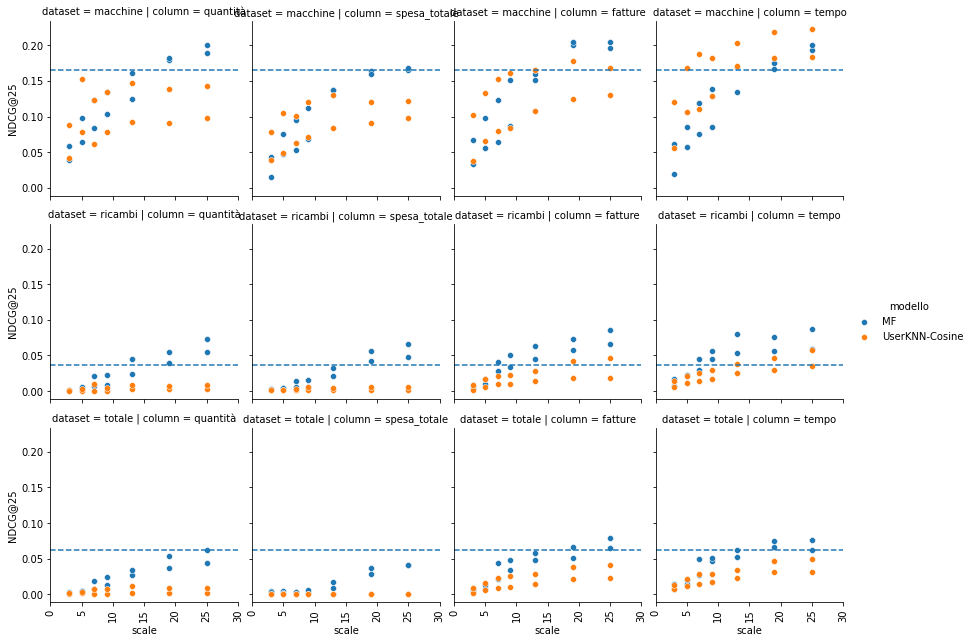
\includegraphics[width=16cm]{figures/prodotto.png}

Possiamo notare come questo approccio fornisca risultati positivi per ciascun tipo di dataset e per quasi tutte le espressioni d'interesse.

\subsection{Fase test avanzata}
Dopo aver visto i risultati delle tecniche nella fase preliminare, si passa alla fase avanzata andando a selezionare tra tutte le matrici dei rating quelle che hanno superato la soglia critica del MostPop. Poi per ciascuna matrice è stato effettuato il tuning dei parametri del modello MF e UserKnn valutato sul validation set, una volta una selezionato il migliore si è proceduto a calcolare il risultato della metrica $NDCG@25$ sul test set.
Nella fase avanzata il nuovo bound era quello del VAECF, quindi ora andiamo a vedere ora i risultati del test set con relativo nuovo bound.\\

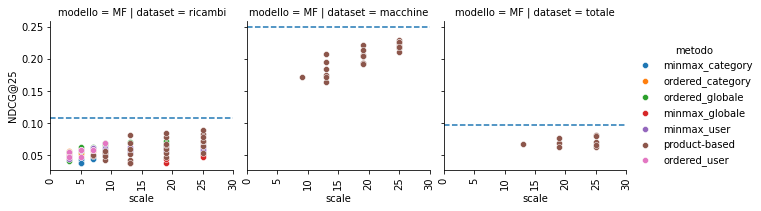
\includegraphics[width=16cm]{figures/validazione_mf.png}

Nel grafico composto dei risultati del test sui modelli MF ottimizzati, le colonne sono rispettivamente il tipo dataset ricambi, macchine, totali con i loro relativi nuovi bound. Possiamo vedere in tutti e tre i grafici i risultati superino di poco il bound e sembra che i risultati miglioi siano prodotto dal metodo product-based.\\

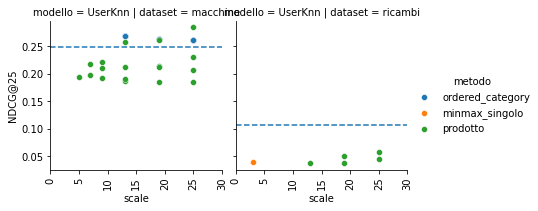
\includegraphics[width=16cm]{figures/validazione_userknn.png}\\
Nel grafico composto dai risultati del modello UserKnn ottimizzato sul test set, le colonne riportano rispettivamente il tipo dataset macchine e ricambi, nel primo primeggia sempre il metodo product-based mentre nel secondo non è presente alcun risultato oltre la soglia.

Per quanto riguarda la distribuzione dei rating nelle matrici, quelle che hanno risultati superiori alla soglia hanno per circa il 66\% una distribuzione gaussian-like. Inoltre per quanto riguarda i valori della scala, i risultati migliori si sono ottenuti con il valore massimo di questa.

Abbiamo quindi tre matrici dei rating prodotte con il metodo product-based con i seguenti risultati sul test set oltre la soglia del VAECF.\\

\begin{tabular}{|l|cccc|}
    \toprule
    $dataset$  & $modello$ & espressione interesse & scala & distribuzione  \\
    \midrule
    macchine & UserKnn& recentezza & 25 & gaussian-like   \\
    ricambi & MF & recentezza & 25 & gaussian-like \\
    totale  & MF & numero fatture & 25 & gaussian-like \\
\bottomrule
\end{tabular}\\

\begin{tabular}{|l|ccccc|}
    \toprule
    $dataset$  & $AUC$ & $NDCG@5$ & $NDCG@10$  & $NDCG@25$ & $NDCG@100$  \\
    \midrule
    macchine &  & 0.1737 & 0.2223 & 0.2844 & 0.3203 \\
    ricambi &  & 0.0777 & 0.0810 & 0.0898 & 0.1428 \\
    totale  &  & 0.0776 & 0.0765 & 0.0808 & 0.1276 \\
\bottomrule
\end{tabular}\\

\newpage
\section{Risultati matrici grezze combinate}
Andremo ora a vedere i risultati delle tecniche basate sulla combinazione delle matrici, si è utilizzato il validation set per il training e il test set per i risultati finali.
Entrambe le tecniche restituiscono risultati simili tra loro e di poco al di sotto di quelli ottenuti con le matrici singole. 

\subsection{Combinazione liste \textit{TopN}}
Questa tecnica, nonostante nell'incrocio macchine - recentezza sembri funzionare, vive di rendita rispetto i risultati delle matrici singole, è stato un fatto un test andando a misurare il coefficiente di similarità delle liste $TopN$ prodotte da ciascun modello e si è visto che è quasi sempre molto alta. Quindi la combinazione delle liste non produce una lista così diversa da quelle di partenza.\\

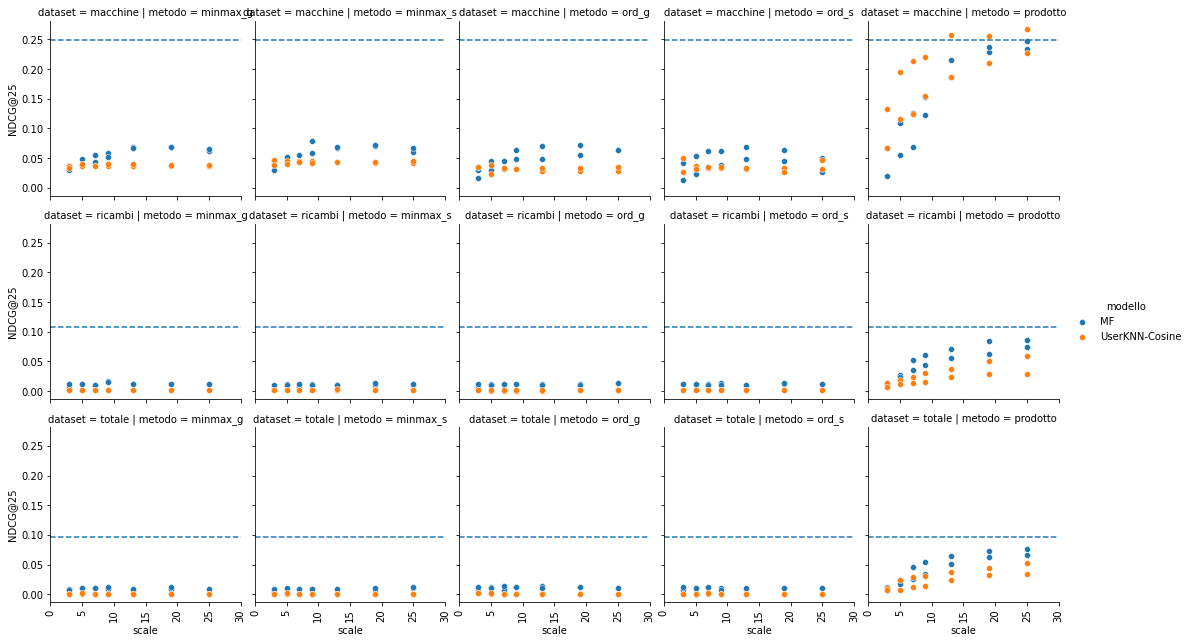
\includegraphics[width=16cm]{figures/comb_1.png}

I risultati migliori ottenuti si attestano per ciascun dataset su questi valori:\\

\begin{tabular}{|l|ccccc|}
    \toprule
    $dataset$ & $AUC$ & $NDCG@5$ & $NDCG@10$  & $NDCG@25$ & $NDCG@100$  \\
    \midrule
    macchine & 0.5658   &0.1516 & 0.2049 & 0.2683 & 0.3041 \\
    ricambi &  0.7873  &0.0756 & 0.0759 & 0.0865 & 0.1427 \\
    totale  & 0.7782   &0.0577 & 0.0648 & 0.0767 & 0.1273 \\
\bottomrule
\end{tabular}\\


\subsection{Media matrici dei rating}
Il motivo per cui la versione basata sulle liste $TopN$ non funziona è che le liste di partenza non sono così diverse dato che molte di esse si basano sull'ordinamento o su una normalizzazione su scala simile, la matrice media ottenuta non è poi così diversa da quella di partenza.\\

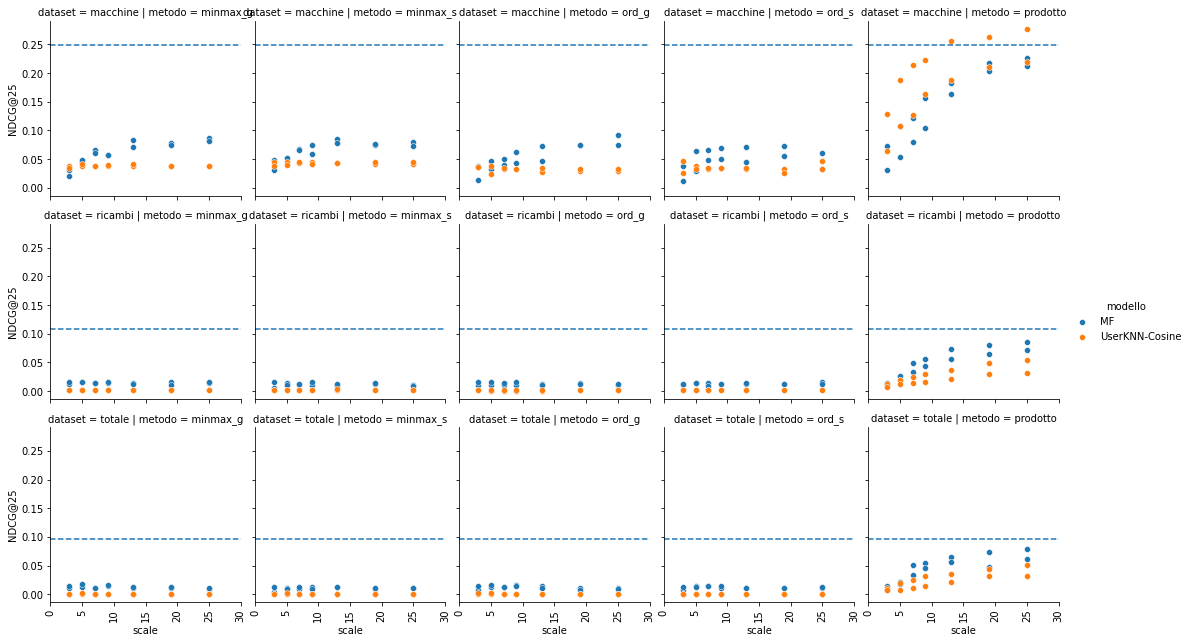
\includegraphics[width=16cm]{figures/comb_2.png}

I risultati migliori ottenuti si attestano per ciascun dataset su questi valori:\\

\begin{tabular}{|l|ccccc|}
    \toprule
    $dataset$  & $AUC$ & $NDCG@5$ & $NDCG@10$  & $NDCG@25$ & $NDCG@100$  \\
    \midrule
    macchine & 0.7288 & 0.1708 & 0.2149 & 0.2775 & 0.3133 \\
    ricambi & 0.8861  & 0.0757 & 0.0766 & 0.0860 & 0.1416 \\
    totale  & 0.8810  & 0.0605 & 0.0649 & 0.0792 & 0.1256 \\
\bottomrule
\end{tabular}\\

\section{Risultati con approccio next-basket}
In questa sezione vedremo i risultati dell'approccio next-based. Per prima cosa andiamo a vedere quali sono stati i parametri selezionati con il tuning per ciascun dataset.\\

\begin{minipage}[H]{0.45\textwidth}
    \begin{tabular}{|l|ccc|}
        \toprule
        $dataset$ &    $\alpha$ &  $q$ & $r$ \\
        \midrule
        macchine & 0.5 & 100 & $\infty$ \\
        ricambi  &	0.75 & 50 & $\infty$ \\
        totale  & 0 & 100 & $\infty$ \\
    \bottomrule
    \end{tabular}
\end{minipage}
\begin{minipage}[H]{0.55\textwidth}
    Possiamo vedere che alla fine il tuning ha portato ad avere una finestra di recentezza  $r = \infty$, quindi stiamo usando la popolarità \textit{popularity user-wise}. 
\end{minipage}\\

Possiamo inoltre vedere che la località $q$ è comunque alta, mentre per quanto riguarda $alpha$ abbiamo che le macchine calcolano la probabilità composta al 50\%, nei ricambi si da più importanza a quella dello user in esame, ed infine nel totale si considera solo la probabilità composta dello user esterno.

Vediamo i risultati sperimentali con i modelli ottimizzati sul validation set:\\

\begin{tabular}{|l|cccc|}
    \toprule
    $dataset$  &  $NDCG@5$ & $NDCG@10$  & $NDCG@25$ & $NDCG@100$  \\
    \midrule
    macchine & 0.5832 & 0.6278 & 0.6506 & 0.6627 \\
    ricambi & 0.1728 & 0.1892 & 0.2381 & 0.3317 \\
    totale  & 0.2196 & 0.2295 & 0.2834 & 0.3653 \\
\bottomrule
\end{tabular}\\

E ora i corrispondenti risultati con il test set:\\

\begin{tabular}{|l|ccccc|}
    \toprule
    $dataset$  &  $NDCG@5$ & $NDCG@10$  & $NDCG@25$ & $NDCG@100$  \\
    \midrule
    macchine & 0.6049 & 0.6476 & 0.6726 & 0.6741 \\
    ricambi & 0.2261 & 0.2403 & 0.2915 & 0.3811 \\
    totale  & 0.1955 & 0.2045 & 0.2595 & 0.3537 \\
\bottomrule
\end{tabular}\\

Ricordiamo che questi risultati non sono confrontabili con quelli delle sezioni precendenti, però i risultati sembrano molti interessanti.